\chapter{Bijection}% by Ahsan Al Mahir}

\begin{linkb}
   \begin{itemize}
        \item \href{https://www.youtube.com/watch?v=Pw0VeDSC_go}{Bijection(Lazim)} 
        \item \href{https://drive.google.com/file/d/1y4aWf4oQsDQvFtwnSwT4JiFHZ_diWT1x/view}{1} , \href{https://drive.google.com/file/d/1zFTQOX1HOWcN1KMPvYR5K2okdZTXP1n1/view}{2}
   \end{itemize}
\end{linkb}

%(This class is taught by following Yufei 
%Zhao's Bijection Note. This note is a great resource for further reading.)


Bijection means a function which is injective  and surjective at the same time. 


\section{Example Problems}
Let you are told to find the number of ways to walk from $(0,0)$ to $(5,4)$. Which is 
called grid walking. It is difficult to find 
the answer unless you find some bijection. 
You may let the right  move $R$ and up move $
U$ which means all the ways are of $RURURRRUU$
 this type. Which is in fact a binary 
 string.  Now it is easier to tackle the  
 problem. And there are $\binom{9}{4}$ ways.


Our next example is about Triangular Grid. 

\begin{example}
A triangular grid is obtained by tiling an equilateral triangle of side length
$n$ by $n^2$ equilateral triangles of side length $1$. Determine the number of parallelograms
bounded by line segments of the grid.
\end{example}
\begin{figure}[ht]
\centering
	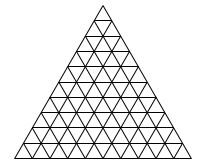
\includegraphics[scale=.5]{tri-grid.png}
	\caption{Three different oriented parallelograms}
\end{figure}
Here observe that there are 3 different types(orientation) of parallelograms.
If you can find the number of parallelograms of a single orientation, by symmetry the total number is thrice the number.

\begin{figure}[ht]
\centering
	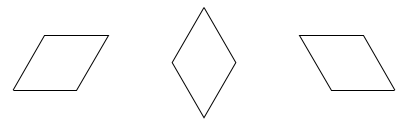
\includegraphics[scale=.5]{parallelograms.png}
	\caption{Three different oriented parallelograms}
\end{figure}
Let us
just count the paralellograms with the middle type of orientation (i.e., no horizontal
sides).

Extend the triangular grid by one extra row at the bottom. The key (and clever)
observation is that starting from any such parallelogram in the original grid, we can
extend its sides to meet the lines to meet the bottom edge of the new row in the large
triangular grid, and there would be four distinct intersection points, as shown below.
\begin{figure}[ht]
\centering
	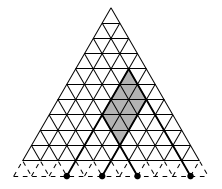
\includegraphics[scale=.5]{tri-grid-sol.png}
	\caption{An added row and the solution}
\end{figure}

Conversely, starting from any four distinct grid points in new bottom edge, we
can extend $60\dg$ lines from the first two points and $120\dg$ lines from last two points
to obtain a parallologram in the original grid. This gives us a bijection between the set
of parallelograms in the original grid with no horizontal sides with set of four distinct
points in the new bottom edge, and hence there must be $\binom{n+2}{4}$ of them. Accounting for
all three orientations, we find that the total number of parallolograms in the original
grid is $3\binom{n+2}{4}$.

(The above solution taken from Zhao's Note.)

\begin{example}
Let $n$ be a positive integer. Determine the number of lattice paths from
$(0, 0)$ to $(n, n)$ using only unit up and right steps, such that the path stays in the region $x \ge y$.
\end{example}
\begin{figure}[ht]
\centering
	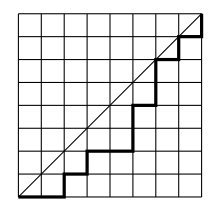
\includegraphics[scale=0.5]{grid-walk-2.png}
	\caption{The Problem}
\end{figure}


We saw previously that the total number of lattice paths from $(0, 0)$ to $(n, n)$ without the $x\ge y$ restriction is equal is $\binom{2n}{n}$. Let us count the number of paths that goes into the $x < y$ region. 
Call these paths |\textit{bad paths}.

Suppose that $P$ is a bad path. Since $P$ goes into the region $x < y$, it must hit the
line $y = x + 1$ at some point. Let $X$ be the first point on the path P that lies on the line
$y = x + 1$. Now, reflect the portion of path P up to X about the line $y = x + 1$, keeping
the latter portion of P the same. This gives us a new path $P'$.


\begin{figure}[ht]
\centering
	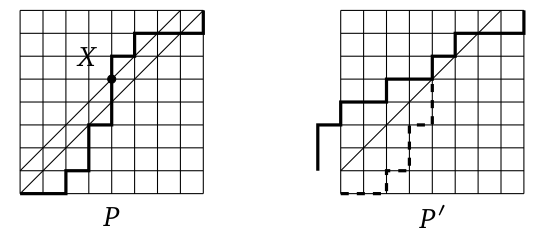
\includegraphics[scale=0.5]{grid-walk-2-sol.png}
	\caption{The Solution}
\end{figure}

We claim that this gives us a bijection between the set of bad paths to the set of
lattice paths from $(-1, 1)$ to $(n, n)$ using only up and right unit steps.

Here is the inverse construction. For any lattice path Q from $(-1, 1)$ to $(n, n)$, let $X$
be the first point on the path lying on the line $y = x + 1$, and let $Q'$ be constructed from
$Q$ by reflecting the first portion of $Q$ up to $X$ through the line $y = x + 1$ and keeping
the rest the same. Then the inverse of the bijection given above sends $Q$ to $Q'$.

To complete the proof of this claim, we need to check a number of details, which
we outline below. The reader should think about why claim is true.

\begin{itemize}
	\ii The inverse construction is well defined. That is, we can always find such a point
	$X$ , and also, the resulting $Q'$ is a always a bad path.
	\ii The two constructions are inverses of each other.
\end{itemize}
The number of bad paths is equal to the number of lattice paths from $(-1, 1)$ to
$(n, n)$ using only unit up and right steps, and there are $\binom{2n}{n+1}$ such paths.

Therefore, the total number of “good” paths, i.e., those that do not go into
the region $x < y$, is equals to 
\[\binom{2n}{n} -\binom{2n}{n+1} = \binom{2n}{n}-\frac{n}{n+1}\binom{2n}{n}=\frac{1}{n+1}\binom{2n}{n}.\]
The above number is called the Catalan Number. There are many more counting problems which are counted by Catalan Numbers.



\section{Practise Problems}
Now you can solve some problems from Yufei Zhao's Bijection Note. This note contains many problems. I am ading some of them.

\begin{problem}
Show that the $n$-th Catalan number counts the number of expressions
containing $n$ pairs of parentheses which are correctly matched. E.g., for $n = 3$,
\[((())) \ \ \ (()()) \ \ \ (())() \ \ \ ()(()) \ \ \ ()()()\]
\end{problem}

A plane tree is an object with the following structure. We start with a root vertex
(drawn at the top), and then with each node we attach a number of new vertices
(possibly none), where the order of the attached vertices matters. For instance, there
are exactly $5$ plane trees with $4$ vertices
\begin{problem}
Show that the $n$-th Catalan number counts the number of plane trees with
$n + 1$ vertices.
\end{problem}


\begin{problem}
Show that the number of ways of stacking coins in the plane so that the bottom
row consists of $n$ consecutive coins is $C_n$ .
\end{problem}



\begin{problem}
Show that the number of triangulations of a convex $(n + 2)$-gon into $n$ triangles
by $n - 1$ diagonals that do not intersect their interiors is the $n$-th Catalan number,
$C_n$.
\end{problem}

\begin{problem}
Let $n$ be a positive integer. Prove that the number of partitions of $n$ equals the
number of partitions of $2n$ with $n$ parts.
\end{problem}
%\section{}

